%   Filename    : chapter_4.tex 
\chapter{Preliminary Results/System Prototype}

\section{Materials}
This study will employ components to gather accurate measurements of reaction time. The device will be composed of one master controller and multiple stations. The study will use the ESP-NOW protocol to achieve wireless connection between the main controller and the stations. ESP-NOW is a wireless communication protocol defined by Espressif which enables multiple ESP based microcontrollers to communicate wirelessly. It is a quick and low-power way to handle connection that is based on the data link layer to achieve faster transmission. The main controller will be the master for the station controllers who will send commands and where data will be gathered and sent to a web-based player development tracker.

\subsection{IOT Components}
\begin{figure}[h]               
	\centering                    
	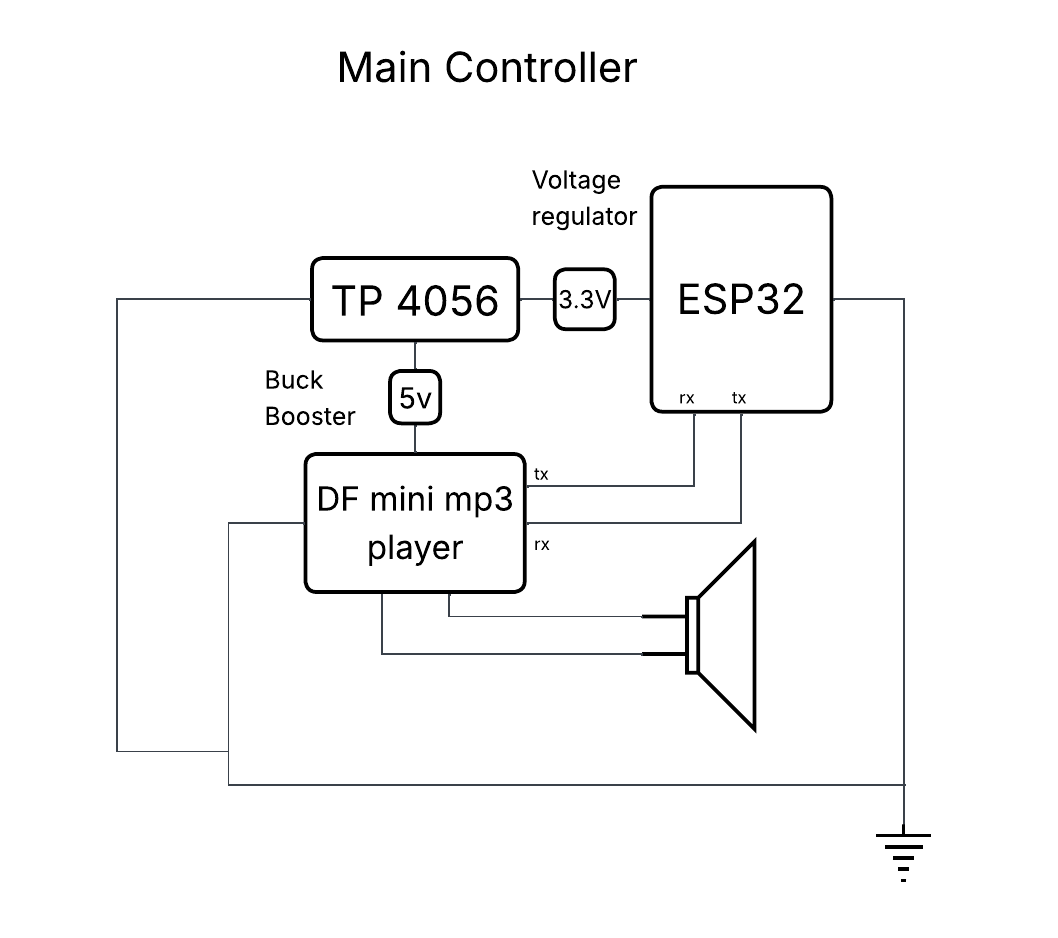
\includegraphics{Master_node.png}      
	\caption{Schematic Circuit Diagram of the Master Controller }
	\label{fig:Master_node}
\end{figure}

In the \figref{fig:Master_node} shows the schematic circuit diagram of the main or master controller. It will use a standard ESP32 controller who will handle the sending of commands to the smaller stations on what they will be performing as well as gathering the data from the stations and sending them to a web based player development tracker where the data will be displayed. A python app will be used to display the data sent by the main controller and will then be uploaded online in the firebase online database. Other components that the main controller has is the DF mini mp3 player module which will be responsible in playing audio sounds for trainings that need audio queue. The audio files will be stored in an SD card for the module to read. It is also connected to a 3W speaker to help amplify the sound it needs. All of these will be powered by an 3.7v 18650 battery. A TP 4056 module  with protection will be used to safely charge the battery without overcharging it. A voltage regulator for 3.3v will be connected from it to stably supply the needed voltage of the ESP32. A buck booster will also be connected to the power source to power the DF mini mp3 module and the 3w speakers.

\begin{figure}[h]               
	\centering                    
	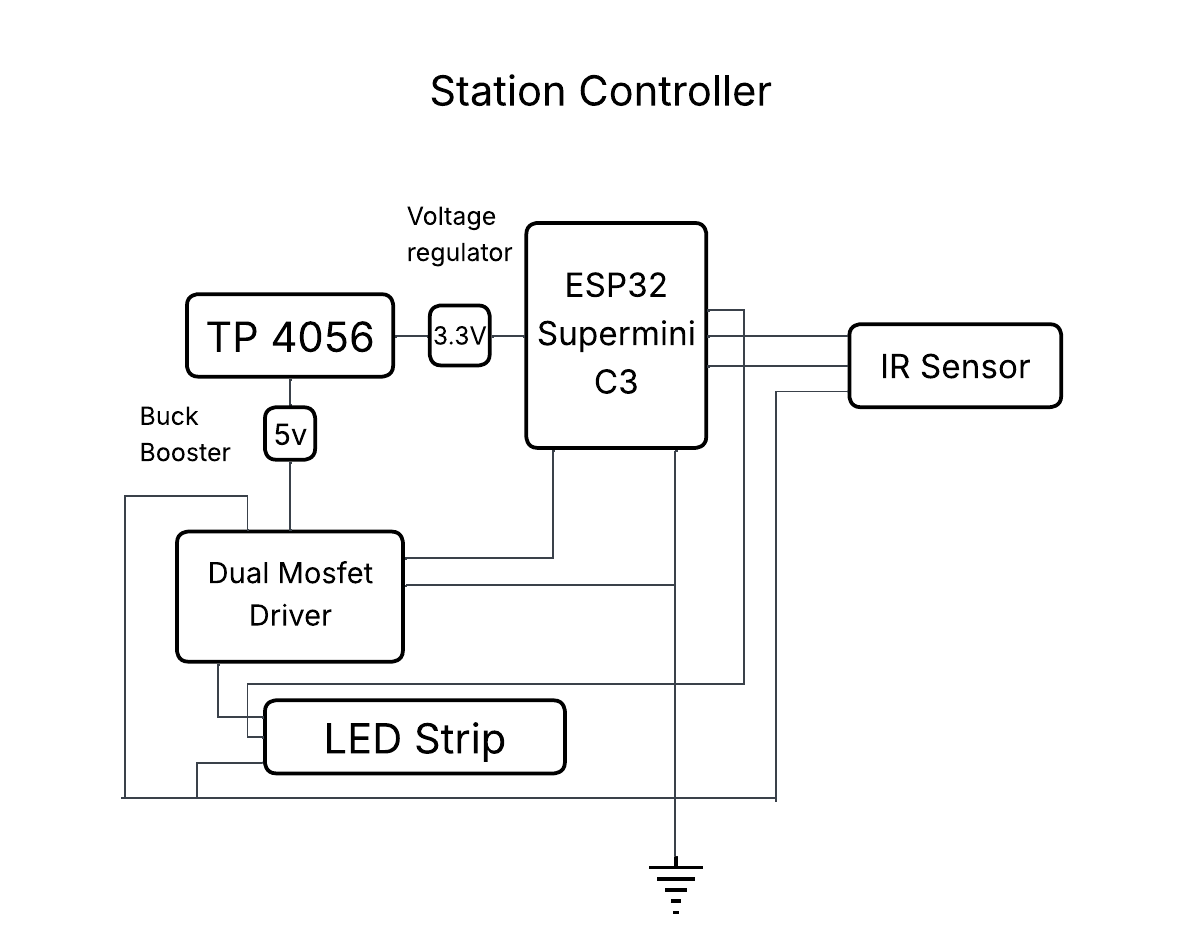
\includegraphics{Station_node.png}      
	\caption{Schematic Circuit Diagram of the Station Controller }
	\label{fig:Station_node}
\end{figure}

For the station nodes, the \figref{fig:Station_node} shows its circuit schematic diagram. An ESP32 super mini C3 is used. It is used as it has a smaller footprint and the sensors needed doesn't exceed the amount of its usable GPIO pins. It will receive commands from the main controller and will execute them. A programmable led strip is connected and will change depending on the command as well as will be turned off by the infrared sensor connected to the station controller. The station controller will then record the reaction time of the performer and will then send the data to the main controller. Similar to the main controller, the station controller will be powered by an 3.7v 18650 battery with a TP4056 module with protection for charging. Again, a voltage regulator for a steady supply of 3.3v will be used to power the station controller and a buck booster for 5v to power the led. The led however will be connected to a dual mosfet driver connected to the station controller to act as a switch for the 5v led strip.
